\section{Proposed Architecture}
A better zoomable representation of these diagrams can be found in the github repository of this project in /doc/pflichtenheft/pics, where also the xml sources are.
\subsection{Overview}

\hspace{-3cm} 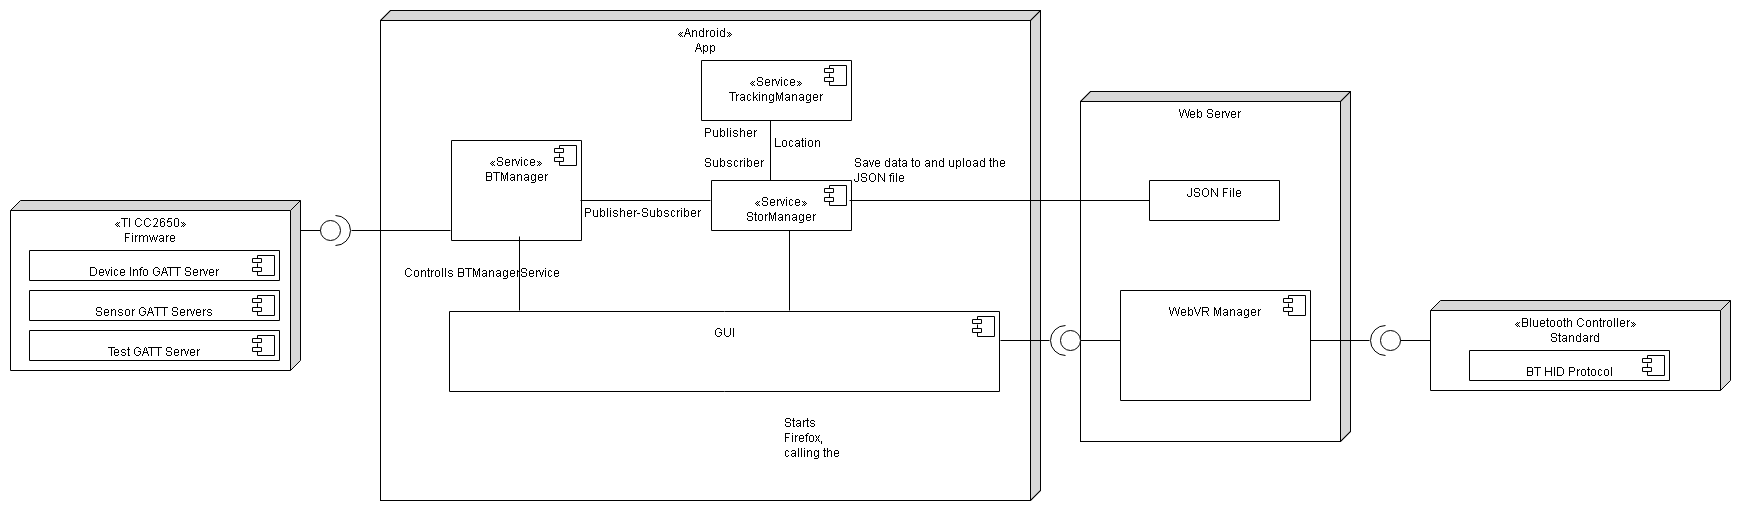
\includegraphics[width=1.4\textwidth]{pics/composite_app.png}


\subsection{Component Decomposition}

\subsubsection{Services}

\begin{itemize}
  \item \textbf{BluetoothManager:} Uses the android.bluetooth and especially the android.bluetooth.le libraries to fetch the sensor data from the sensor device. \\
  
 \hspace{-4cm} 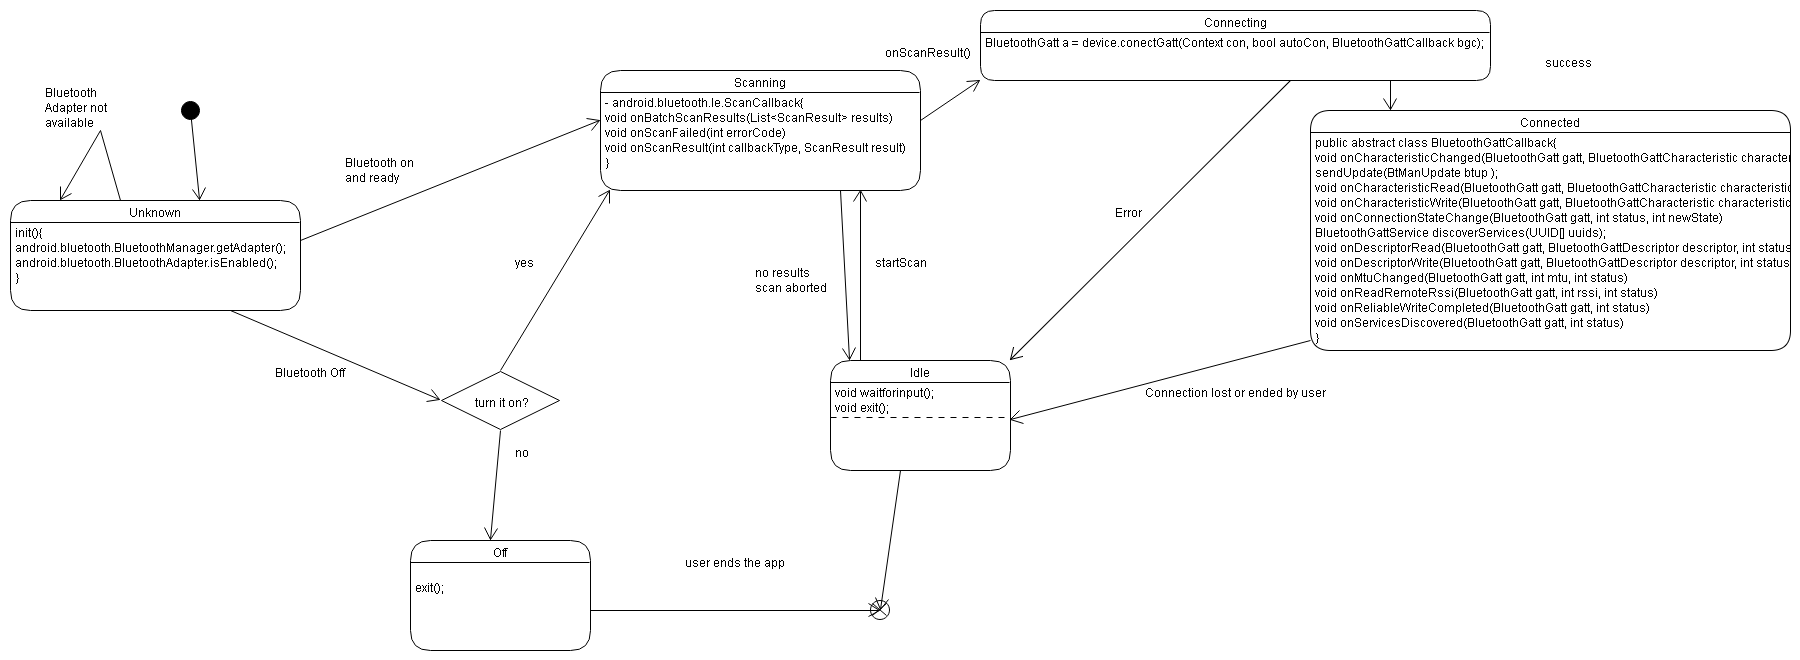
\includegraphics[width=1.4\textwidth]{pics/bt_state.png}
  
  \item \textbf{TrackingManager:} Handles the tracking of the (current) location where the data are recorded. The current position is determined by GPS and enhanced by the cellphone sensor and wifi data.

 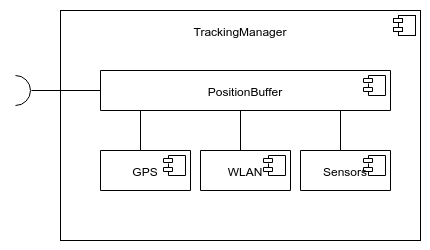
\includegraphics[width=0.8\textwidth]{pics/TrackingManager_Composition.png}

  \item \textbf{StorageManager:} Processes the data provided by the TrackingManager and the BluetoothManager. Uses a JSON file to store data.

 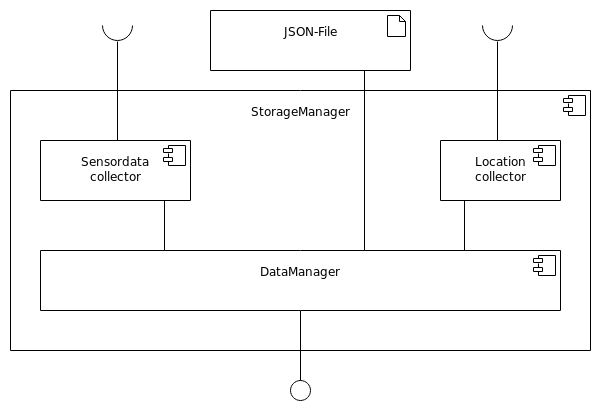
\includegraphics[width=0.8\textwidth]{pics/StorageMgr_Composition.png}

  \item \textbf{WebVRManager:} Handles the display of the virtual reality scene and the given data from the sensor.
  
 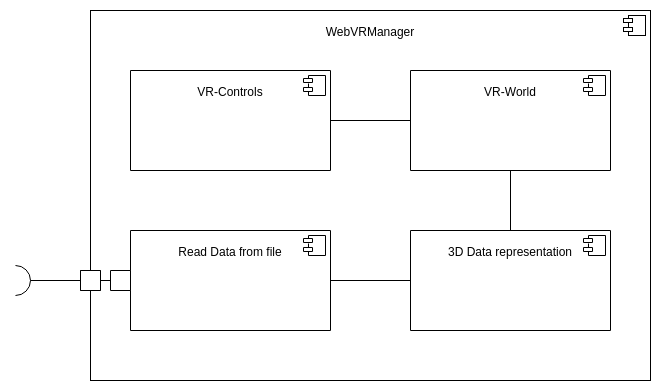
\includegraphics[width=0.8\textwidth]{pics/WebVRManager.png}

\end{itemize}

\subsubsection{GUI}

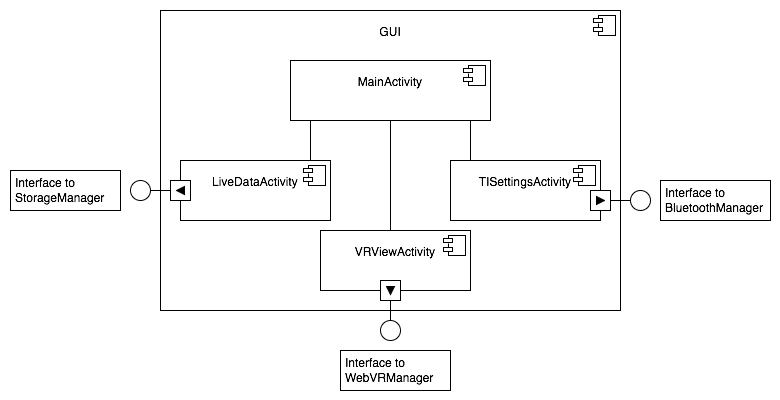
\includegraphics[width=0.8\textwidth]{pics/GUI.png}

\begin{itemize}
  \item \textbf{MainActivity} Provides the main startup screen as the main entry point.
  \item \textbf{VRViewActivity} Shall open a new browser window to display the WebVR webpage.
  \item \textbf{LiveDataActivity} Shall provide a view of the sensor data in human readable form.
  \item \textbf{TISettingsActivity:} Shall provide a settings screen containing scanning and connecting, connected devices and device settings fragments.
  \begin{itemize}
    \item \textbf{ScanningConnectingFragment} shall show the scanning results, delivered by the SensorTagBluetoothReceiverService and provide a connect on/off control.
    \item \textbf{ConnectedDevicesFragment} shall show the connected devices and a short info about the current setting and state of the sensor device.
    \item \textbf{ConnectedDevicesSettingsFragment} shall implement the configuration of the app features of the sensor.
  \end{itemize}
\end{itemize}

\subsubsection{Additional Classes}
\begin{itemize}
  \item \textbf{GATT Profiles} (for each sensor one)
  \item \textbf{GATT Sensor Service UUIDs}
  \item \textbf{Parser Functions} because the BLE protocol implemented in the TI CC2650 delivers raw sensor output
\end{itemize}

\subsection{Hardware/ Software mapping}

TO DO ???